\chapter{Design}
\label{chapt:design}
This chapter presents the design of MultiChain and how it was implemented.
The first thing that will be introduced is how MultiChain is implemented within Tribler
to outline the context of the design and implementation.
The contents of blocks are presented and how they form chains in MultiChain.
We will cover the creation of blocks and the multiple implications of the chosen design.
We will explain how MultiChain adresses the freeriding problem.
Additional pheripheral systems that work with MultiChain are also explained.

Tribler uses communities to add functionalities to peers.
New communities are packaged into new Tribler versions.
These versions are downloaded by peers.
A community provides a set of messages and endpoints for other peers.
The community can communicate with the endpoints of other peers as well and send a message to these endpoints.
Other peers are automatically discovered using Dispersy.
Examples of communities are the TunnelCommunity that adds functionality to download anonymously~\cite{Plak-anonymous,tanaskoski-anonymous}
or the AllChannelCommunity to distribute torrent files.
Our system will be implemented by adding a new community to Tribler.

The MultiChain community can be run standalone,
but its main use is to integrate with Tribler and track up and download amounts for torrents.
It aims to replace the current reputation system Bartercast in the future.

\section{Datastructure design}
In this section we wil describe the design of the chains inside MultiChain.
We will first describe the contents of a single block.
Next, we will explain how blocks are chained together for a single peer.
These chains are intertwined and we will clarify this entanglement.
Finally, we will describe how the blocks provide security against tampering.

\subsection{Bookkeeping}
A peer will upload to and download from other peers in the network.
The peer A will want to increase its reputation and have a transaction transcribing his contribution.
A will initiate the process to create a block with peers that he has uploaded to.
These peers will be referred to as B.
The contents of a block can be seen in Figure \ref{fig:block}.
Every block only contains one transaction.

\begin{figure}
	\centerline{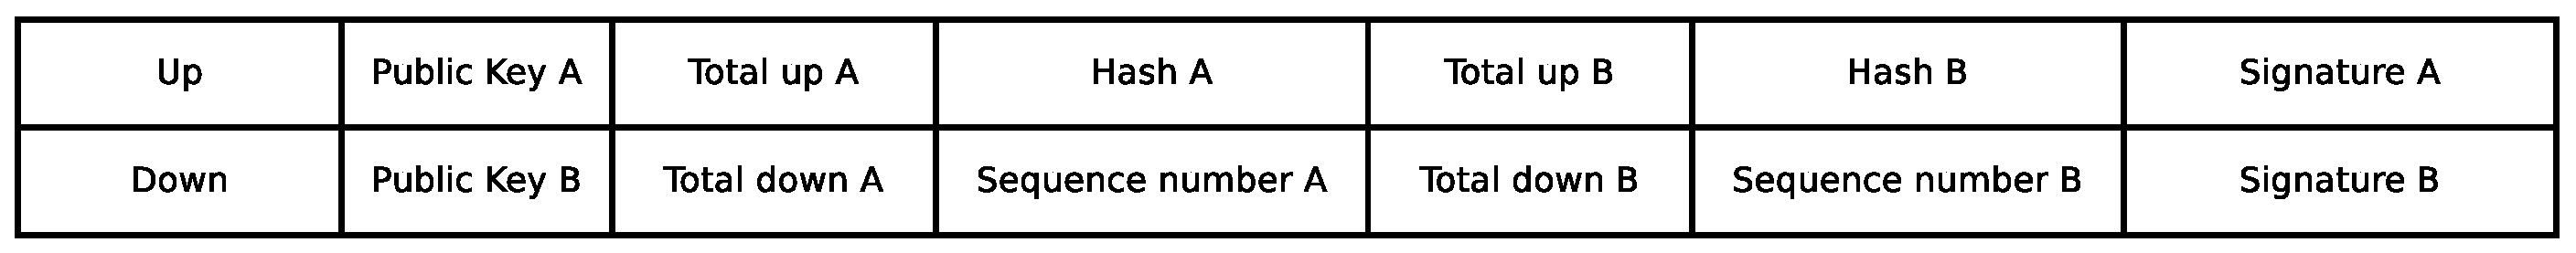
\includegraphics[scale=0.3]{design/figs/block.eps}}
	\caption{A block in MultiChain.}
	\label{fig:block}

\end{figure}

The up and down represents the amount that has been transferred between A and B directly for the current transaction.
Up means data uploaded by A and down the data downloaded by B.
Every peer in Dispersy has a public and private key and are unique identifiers.
A block contains both public keys of the peers,
so it is possible to verify to which peers the transaction belongs to.
The total amounts of A and B is added to the block.
This is the amount summed across the whole chain of A and B respectively.

The blocks are linked to previous blocks by adding the hashes of the previous blocks of both peers.
This creates a directed acyclic graph of blocks.
An overview of a chain of blocks is seen in Figure \ref{fig:transaction-chain}.
In this overview the chain of B is currently ignored.
The first block references a special genesis hash identifying the block as the first block.
A block has two sequence numbers, one for A and for B.
These numbers allow blocks to be ordered without having to walk across the hashes linking the blocks together
Both peers add their signature to the block to announce that they approve the contents of the block.

\begin{figure}
	\centerline{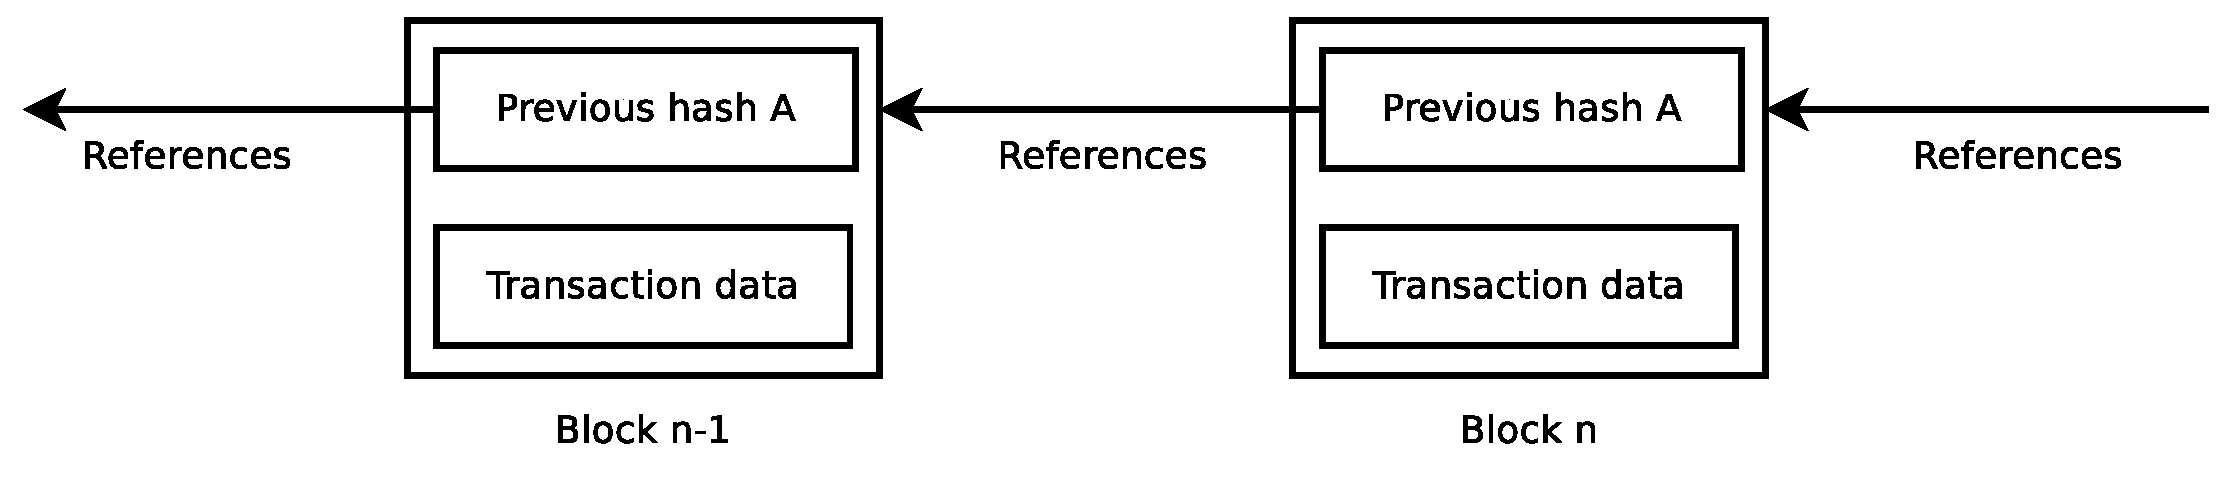
\includegraphics[scale=0.3]{design/figs/transaction-chain.eps}}
	\caption{A chain of blocks in MultiChain.}
	\label{fig:transaction-chain}
\end{figure}

\subsection{Scalable reciprocity}
\label{sect:scalable-reciprocity}
One of the main pillar of the design is to have a transaction history for every peer.
The reasoning behind the idea to abandon a global, full transaction history
is that it will always become the bottleneck in the system.
This will limit the amount of interactions that can be processed.
Before this limit is reached, less powerful machines are already excluded in participating.
For example, a global, full transaction history is the block chain of Bitcoins, discussed in section \ref{sect:bitcoin}.
The block chain already shows these limitations.
Commonly, this way of design is used to prevent double spending.
We believe that it is possible and much cheaper to detect and punish double spending than prevent double spending.
This will be described in section \ref{sect:branch}

The reason for the limitation is that every interaction will have to be distributed to every peer in the network.
Every transaction has to be processed by every node at the cost of bandwidth, computation power and storage.
The cost might be very limited for a single transaction,
but with greater scale these costs will add up when the amount of transactions are increased.
The amount of these three resources is limited and will limit the amount of transactions that can be processed.
This problem can be seen to affect Bitcoins and has been demonstrated in section \ref{bitcoin-limit-size}.

Every node has its own transaction history and only needs the transaction history of the peers it interacts with.
Within MultiChain peers can try to congregrate the full transaction history or only a subset
This flexibility provides MultiChain with unbounded scalability for the network as a whole.
Low-powered devices will be able to keep participating
as long as they have enough power to process the transactions relevant to them.

\subsection{Entanglement}
Chains become entangled, because every block is shared between peers.
Every block is present in two chains and references the previous block of node A and of node B.
The chains quickly form a large graph with every node in the graph representing a block.
Every node has two outward directed edges and two incoming directed edges
except the nodes representing the genesis block and the most recent block.
The outward edges point to the previous blocks
and the incoming edges come from the next block in chronological ordering.

An simple example of three blocks can be seen in Figure \ref{fig:chain-example}.
In this example the first block contains a transaction between peer A and B.
This block references the previous block of both A and B.
Peer A continues with a transaction with C and peer B transacts with D.
Now the previous hash of A and B is the same as they share a block on their chains.
This hash is used in different transactions.
Color has been added to denote the direction of the chain of peers.

\begin{figure}[ht]
	\centerline{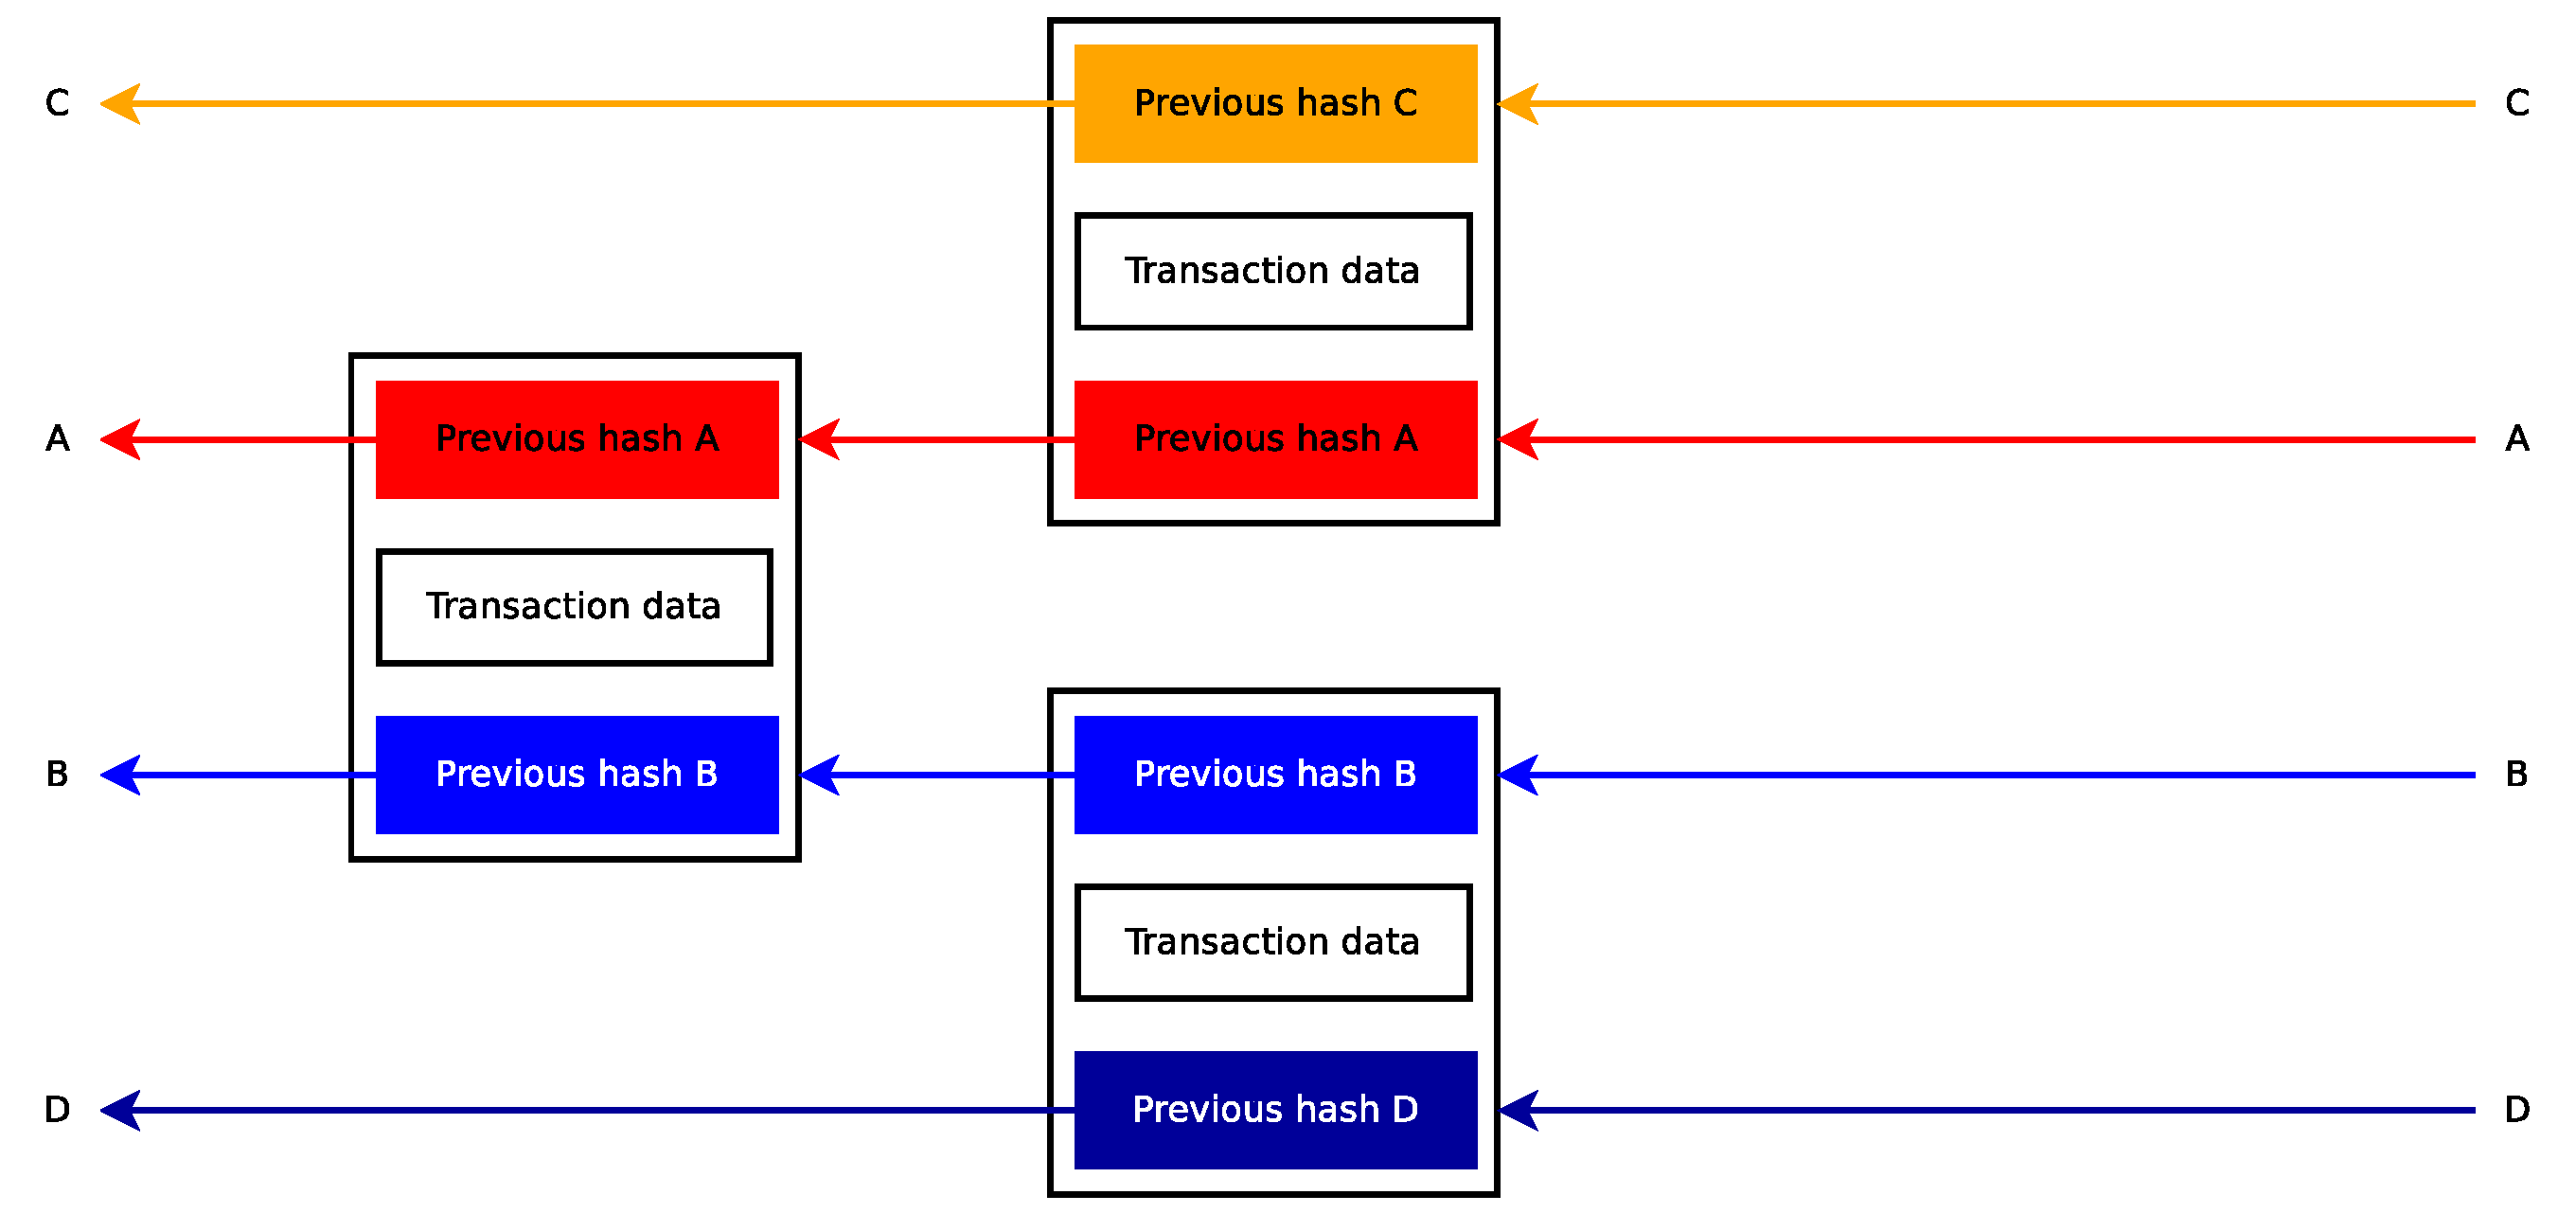
\includegraphics[scale=0.3]{design/figs/entangled-chain.eps}}
	\caption{Entanglement of chains within MultiChain.}
	\label{fig:chain-example}
\end{figure}



\subsection{Protecting the blocks}
\label{sect:repudiation}
The blocks have to be cryptographically protected and validated.
Tampering with the contents of blocks should be detectable and useless.
In part this is already done by using the hashes as pointers in subsequent blocks.
If a block in a chain is changed, then the subsequent hash pointers will become invalid~\cite{VanderLubbe-crypto}.
The chain becomes detached.

A second issue is that peers should not be able to deny conducting a transaction.
This will prevent a peer to be able to deny his freeriding if this is transcibed in his chain.
Both peers sign the block using their private keys to acknowledge that the transaction has happened.
This signature is added to the block.

In a transaction between peer A and peer B, the whole block is not signed by every peer.
Peer A can only make valid claims about, and have authority, over the interaction between peers
and his own total up and download amounts.
So A does not need to sign the data containing the previous hash and the total up and down of the other peer B.
These amounts can be verified using the chain of peer B.
The parts of what is signed by peer A and what is signed by B can be seen in Figure \ref{fig:signatures}.
\begin{figure}
	\centerline{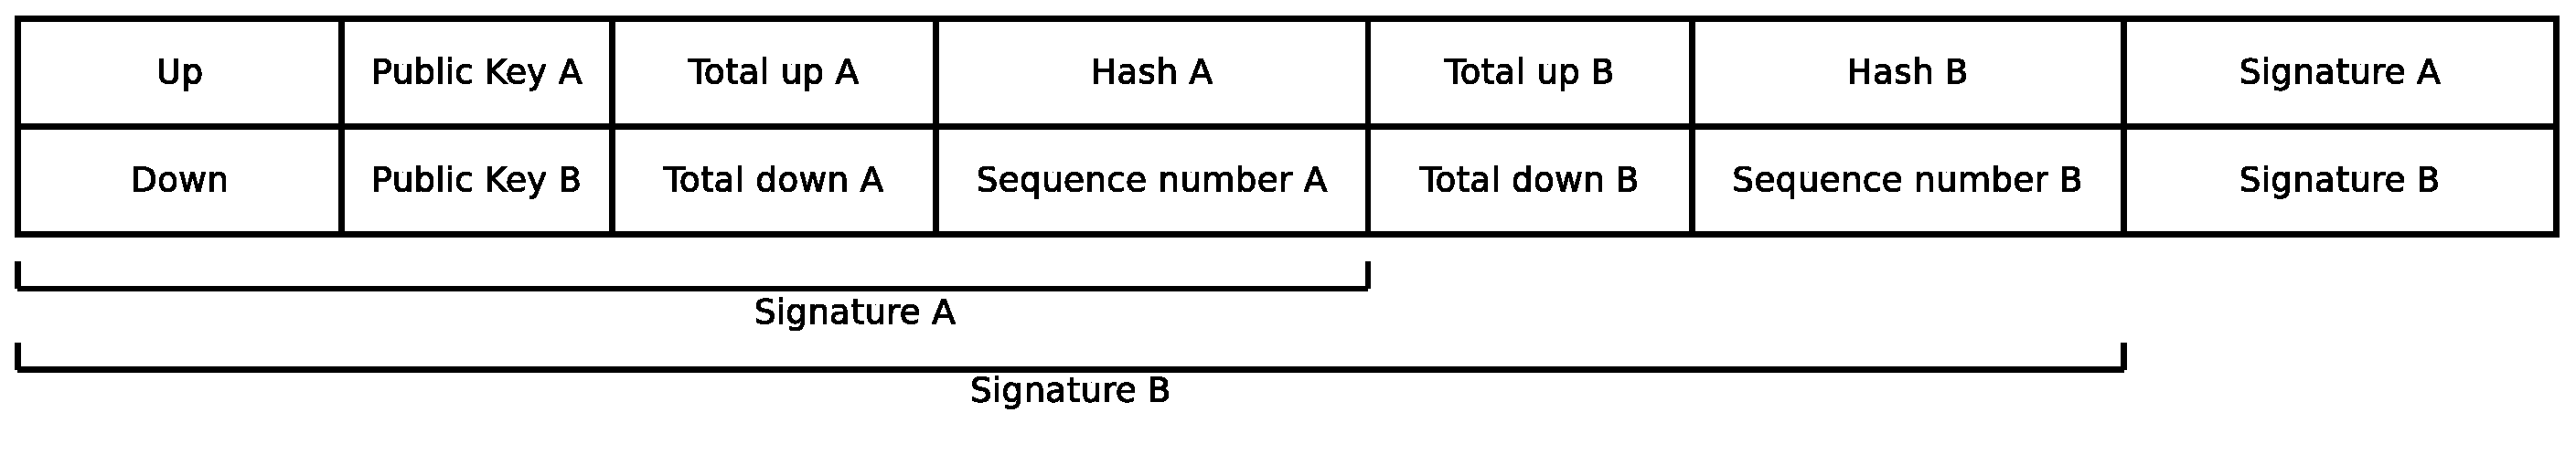
\includegraphics[scale=0.3]{design/figs/signatures.eps}}
	\caption{Fields protected by each of the two signatures.}
	\label{fig:signatures}
\end{figure}

Digital signatures have the property to be non-repudiable of origin~\cite{VanderLubbe-crypto}.
After signing a block the signer cannot later deny providing his signature.
Only with the possesion of a secret key,
a signature can be made;
so only the signer could have made the signature.
This is assuming the secret key was not comprimised.
The blocks become durable records and are irrevokable and irrefutable.
Because peers cannot repudiate their own signature.



\section{Block creation protocol}
\label{design:block_creation}
In this section we will explain how blocks can be created with a simple design
that will limit and expose freeriding.
Afterwards, we will explain a fundamental problem with creating blocks in an asynchronous system.
This problem is present in the simple design
and we will describe how MultiChain deals with this problem.

\subsection{Exchanging signatures}
Two peers in a network will create their blocks together without having to rely on a third party.
Between the peers one is uploading to the other.
The uploader is traditionally called the seeder in BitTorrent and the receiver of this data the downloader\cite{Cohen-bittorrent}.
The seeder will initiate the block creation.\,
co the seeder can decide how altruistic it wants to be towards the downloader regarding its collaboration.
We will explain how the block creation protocol works.
A sequence diagram can be seen in Figure \ref{fig:exchange-new-sequence}.

\begin{figure}[tpb]
\centering
\subfigure[Sequence diagram for block creation]{
\centerline{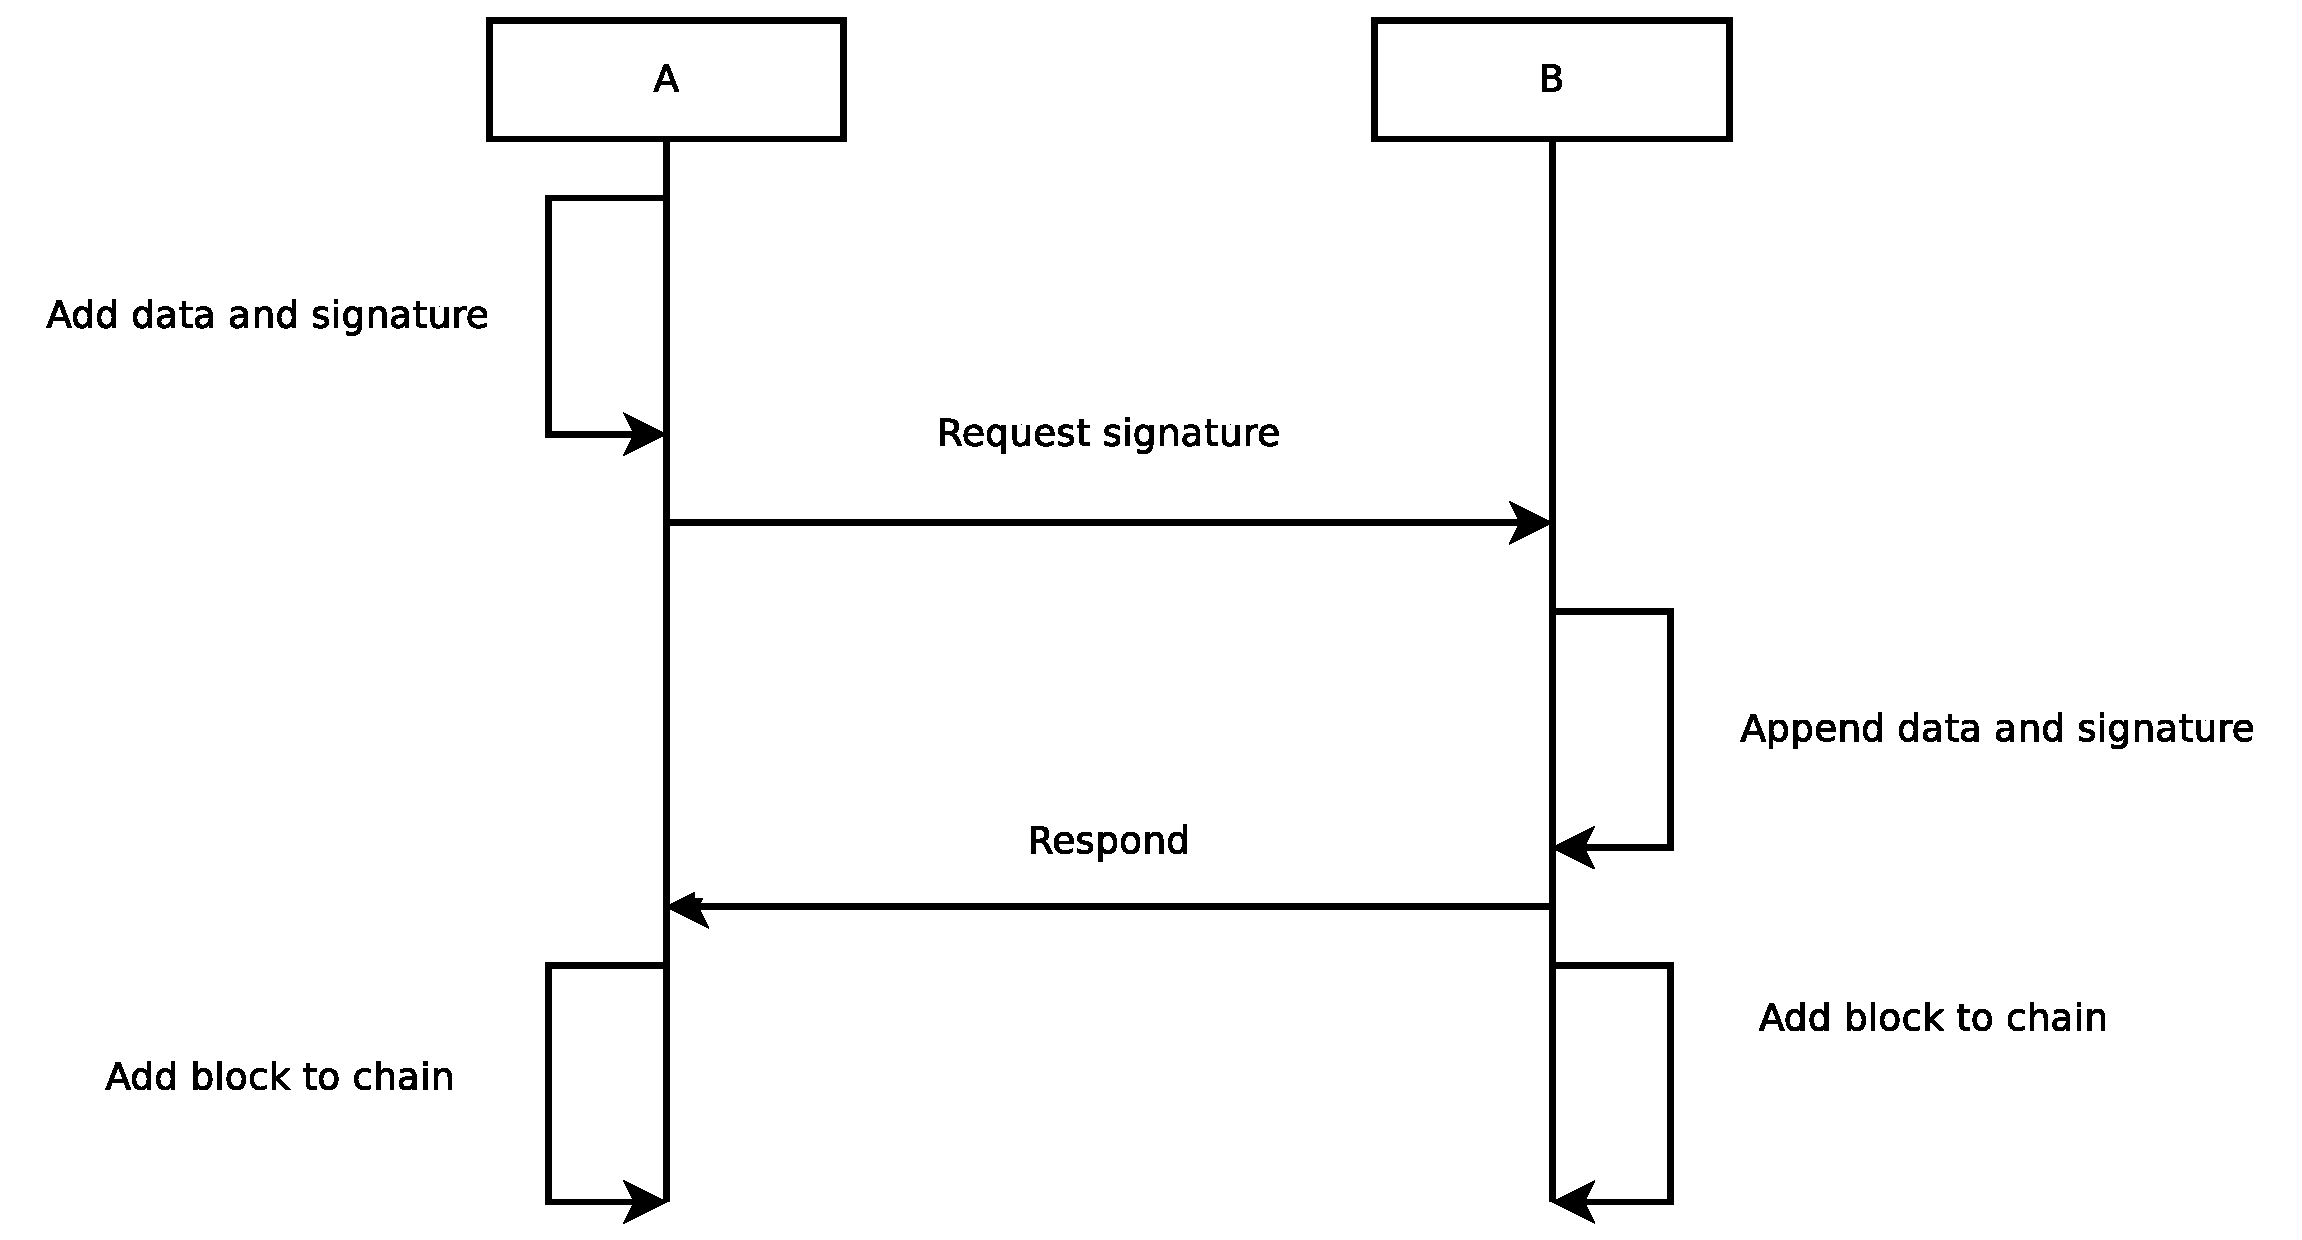
\includegraphics[scale=0.3]{design/figs/exchange_new.eps}}
\label{fig:exchange-new-sequence}
}

\subfigure[Data added by peer A and B for a new block.]{
	\centerline{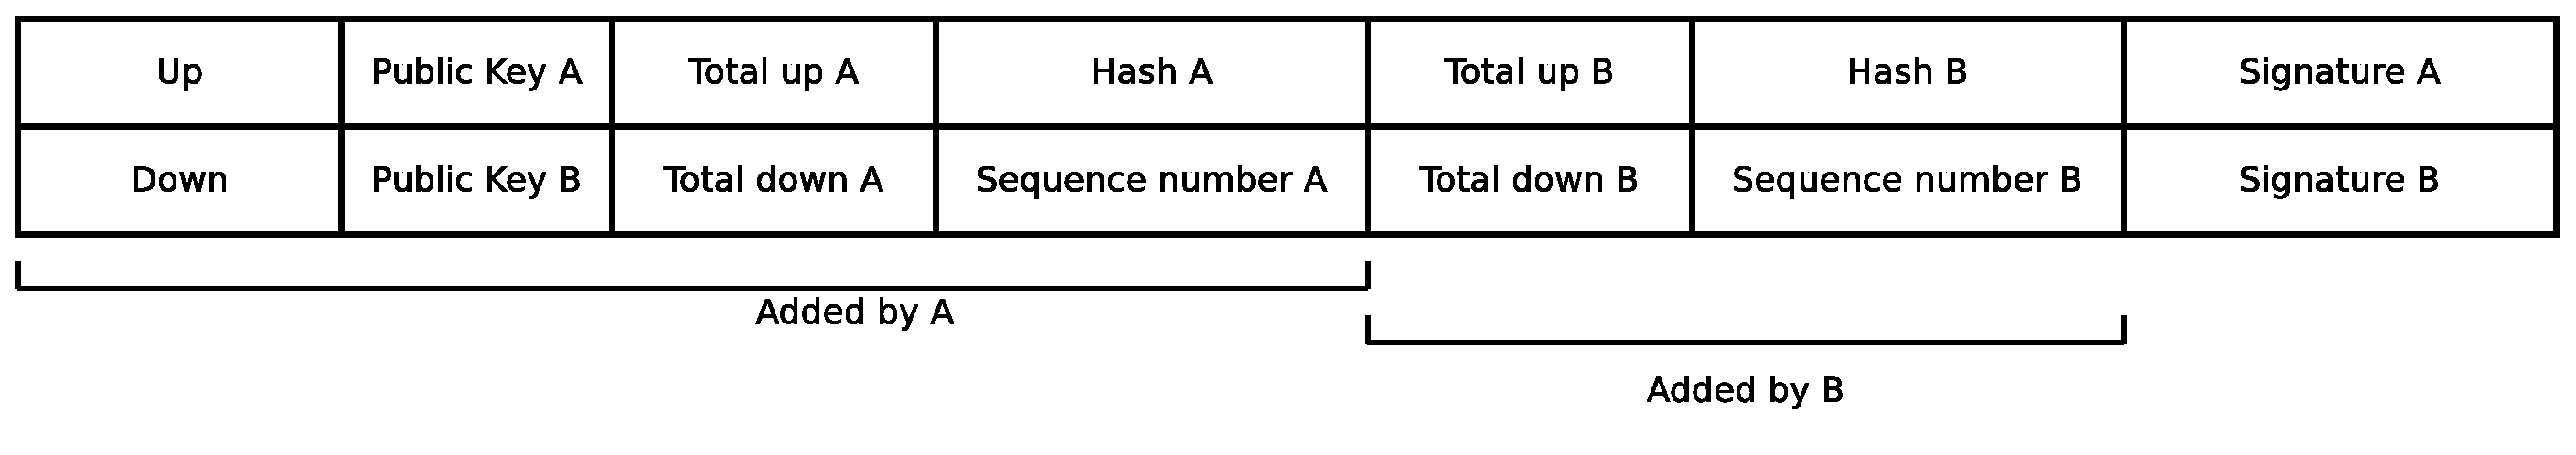
\includegraphics[scale=0.3]{design/figs/packet_creation.eps}}
\label{fig:packet-creation}
}
\caption{Exchanging data for block creation.}
\label{fig:block-creation-new}
\end{figure}

The seeder, A, will create a packet that will be sent to the downloader, B.
A will add to this packet the data uploaded and downloaded data between the peers
that has not yet been added to the MultiChain.
It will add these amounts to its total uploaded and downloaded data
and add these total amounts aswell to the packet.
Finally, it adds the public keys of both peers and its own hash pointer to the packet.
This packet is signed using its private key and sent to the downloader.
The data that A adds can be seen in Figure \ref{fig:packet-creation}.

B will receive this packet and check if the amounts are correct, if the signature is correct,
and if A has not used the previous hash before.
If this is all correct,
then B will add the amounts of uploaded and downloaded data to its own total amounts.
The data contained in the previous packet, the total amounts of B and the hash of the previous block is
inserted into a new packet.
This packet is signed by the private key of B and sent back to A.
The data that B adds can be seen in Figure \ref{fig:packet-creation}.

Both parties now have the data of the block and can add this to their chain and continue forward.
A does this upon receival of the block.
B does this immediatly after sending the return packet to A.
At this point a new block is created.

\subsubsection{Integrating with Dispersy}
\begin{figure}[!h]
\centering
\subfigure[Sequence diagram for block creation.]{
\centerline{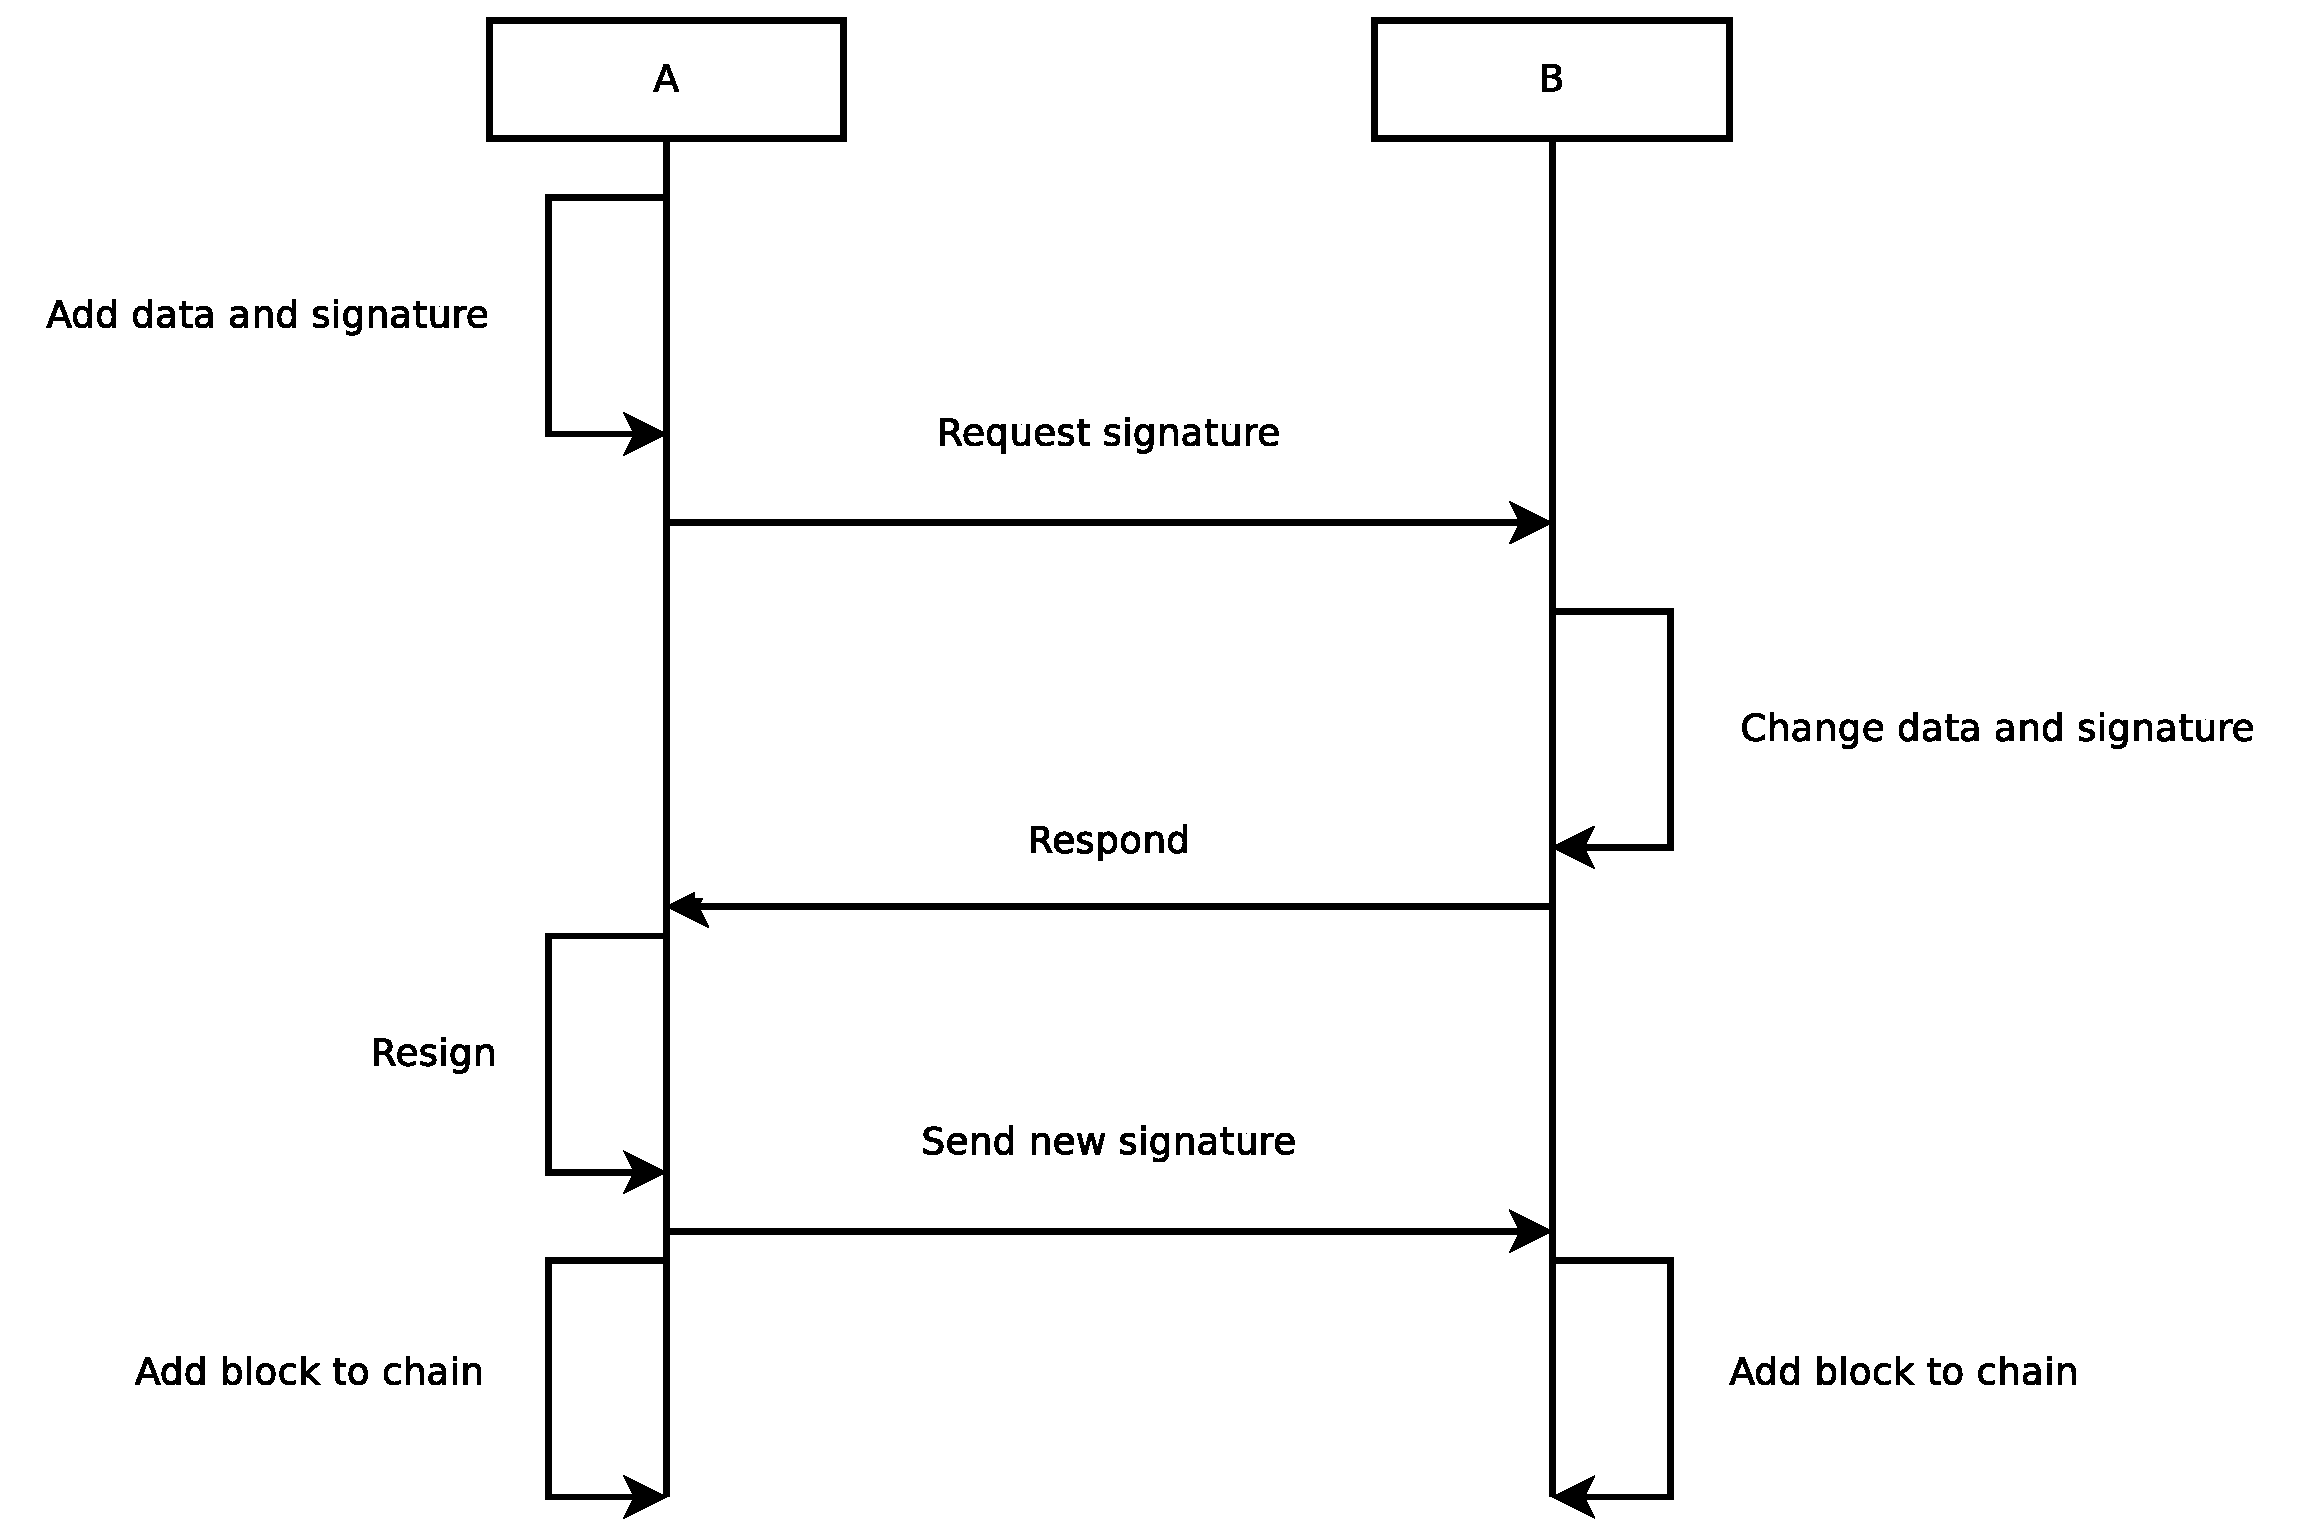
\includegraphics[scale=0.3]{design/figs/exchange_old.eps}}
\label{fig:exchange-old-sequence}
}

\subfigure[Data added by peer A and B for a new block.]{
	\centerline{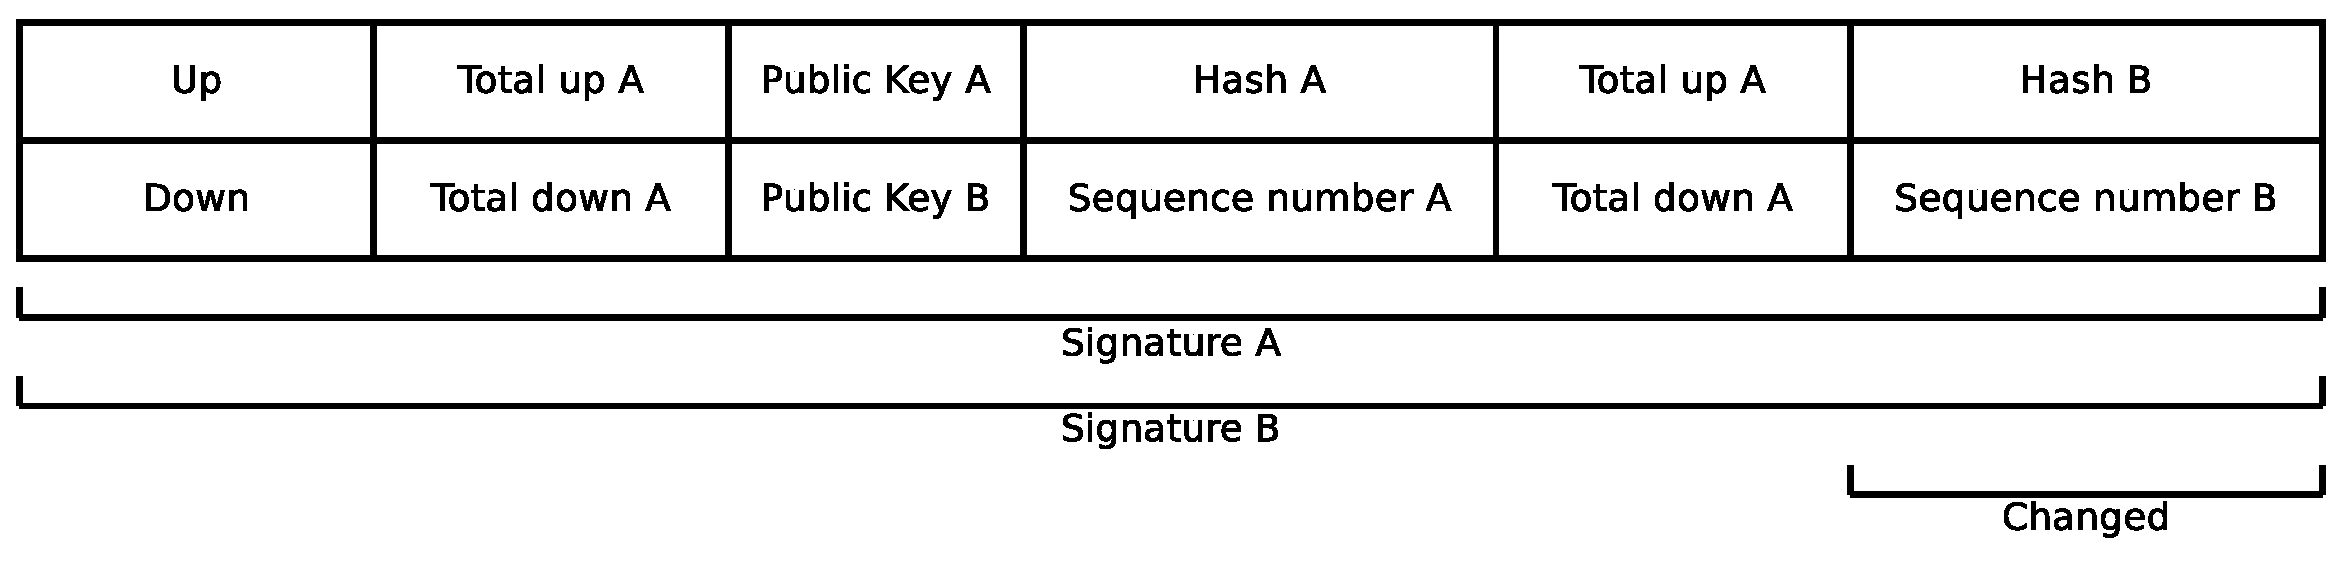
\includegraphics[scale=0.3]{design/figs/signature_old.eps}}
    \label{fig:payload-signature-old}
}
\caption{Exchanging data for block creation using existing functionality.}
\label{fig:block-creation-old}
\end{figure}
Within Dispersy functionality was already build to create a message, sign the message
and request multiple nodes to also provide their signature on this message.
This existing functionality could be used by MultiChain to exchange signatures
between A and B for the creation of a new block.

A would initiate a message, insert its data into this message, sign the message, and send this message to B.
The functionality would allow B to accept the message and provide its signature or
modify the message and then provide its signature.
Only B knows the hash of its head node, and the total up and total download metrics.
So B will always modify the message and insert its own data in the message.
But this would invalidate the signature of A,
because the signature of A was also placed on the empty part of the message where the data of B is inserted.
The contents of the message and who signs what can be seen in Figure \ref{fig:payload-signature-old}.

After B returns the message,
A would have to resign the message.
But B also needs this valid signature from A before it can add the block to its own chain.
So A would need to send a third message to with the new, valid signature back to B.
A sequence diagram can be seen in Figure \ref{fig:exchange-old-sequence} of how it would work in Dispersy.
Functionality was added to Dispersy that allows to append data in a signature request.
This allows the full signature exchange to be achieved within two messages.
\input{design/limitingfreeriding.tex}
\subsection{Synchronization problem}
This design does have one major problem with synchronization.
It can never be decided in an asynchronous communication model
if the other node will ever respond and when it will respond.
The proposed block by A only needs an interaction of B to be finished
and B can finish this transaction at anytime that B decides upon.

But the future block contains an immutable hash pointer
to the previous block in the chain of node A.
So while this transaction for a potential block is outstanding,
node A cannot interact with any other node C to create a different block.
If it would, then B could ultimately respond and a branch with different blocks
would be created for the chain of A.
This simple design introduces therefor an external response dependency problem.

The to-be-designed system has to be fault tolerant to
common problems in a challenged network, such as node failure.
A second design goal is to be able to process transactions quickly and on a large scale.
These design goals prevent the adaption of a simple design that will halt until node B responds.
This design would also result in a deadlock situation, as explained in section \ref{sect:deadlock}
We will explain three possible design solutions to this problem.

\subsubsection{Fair exchange signature scheme}
A fair exchange signature scheme (FESS) allows two players to exchange digital signatures in a fair way.
Fair constitutes that no player can take advantage of the other.
Either both players receive each others signature or no player receives the other's signature.
It is infeasible for a node to acquire a signature without giving up their own signature.\cite{asokan-fairexchange},
a FESS could be implement for the fair creation of the block.

But currently all known FESSs use a trusted third party (TTP) at some point\cite{asokan-fairexchange}.
Some schemes exist that are optimistic and will only need a TTP to resolve conflicts.
But any TTP will not adhere to the Tribler philosophy
of being a truly fully distributed peer-to-peer system.
The TTP will introduce a central point of trust and a scalability bottleneck.

\subsubsection{Reverse repairing of chain}
Another potential solution would be to rework part of the chain.
The creation of block could be deemed to have failed by node A.
If at a later point the block is still created by B,
then the block could be reworked back into the chain.
This would require every hash pointer to be updated afterwards.
If these hash pointers are modified, then the signatures are invalid.
Every signature would have to be renewed and requested at every node.
This is unscalable if nodes needs to rework many blocks and can clog the system.
These nodes can possibly no longer respond and would result in new invalid blocks.

\subsubsection{Half signed blocks}
\label{des:halfsigned}
The chosen solution is to keep it simple and allow for inconsistencies between the chains of A and B.
It will be shown that when an inconsistency does occur, this is in favor of A.

When node A sends a signature request to B,
then A will be optimistic and will wait for B for a timeout period.
During this time, A will not interact with another node C.
But if A does not have to interact with node C after the timeout period,
then A will still accept a response of B.
There are three potential scenario's of what will happen to the message.

\begin{enumerate}
\item
In the normal situation, node B will respond in time to the message.
B will send back the message
and both A and B will have added the same block in their own chains.
This situation also occurs if A has timed out,
but has not yet interacted with another node C.

\item
Node B can be malicious or simply have failed and B will never respond.
Node A will timeout, add a half signed block to the chain and can continue interacting with other nodes C.
A will have to decide how to react upon B not responding.
A possibility would be to stop helping B.

\item
The response of B can also be late.
After B has received the request by A,
B will create a block and adds this block to its chain.
B will send its response to A,
but the message will arrive too late at A.
A will have timeout and  will ignore the message.
The block is not added to the chain of A.
\end{enumerate}

The last scenario is the most complex and requires additional clarification.
A initiates the signature request and therefore the block will be favourable for its reputation.
Because this is a reputation system, this inconsistency is an allowable comprimise.
In a currency system, this comprimise would not be allowable.

The design is scalable as it will not force a node to wait too long for a failed node
and will try to interact as fast as possible with other nodes.
A small grace period can be used to allow node B to have enough time to respond in a normal manner.
No trusted third party is introduced so a distributed design is achieved.

\section{Single operations on the chain}
\label{sect:deadlock}
Inside a chain only a single block of a peer is allowed to point to a previous block.
A peer cannot have multiple blocks belonging to him all pointing to the same previous block.
As this is a potential attack as described in section \ref{sect:branch}.
The chain of a peer can only be moved forward by a single block at any time.
Only after a new block is created is the new hash available to be used in the next block.

To ensure this happens correctly the MultiChain community contains mutual exclusive code
that excludes any new operations on the chain if an operation is already pending.
The mutual exclusion is achieved by having to acquire an atomic token to allow to perform an operation on the code.
The MultiChain community will receive incoming signature requests
or requests by other parts of Tribler to send out an outgoing signature request.
The community will decline this request if the token is not available
returns execution to other parts of Tribler.
The token can be unavailable while waiting on another peer in the network to finish responding to a signature request.

\subsection{Circular dependency on the token across peers}
When a MultiChain peer has a pending signature request,
then the peer itself will not respond to incoming signature requests from other peers.
These peers themselves will also not respond as they have a pending signature request.
This can create a circular dependency on the availability of the token.
If two peers send a request to each other at the same time, they will wait on each other.
This could result in a deadlock.

MultiChain prevents this deadlock to occur by allowing a transaction to fail
as explained in section \ref{des:halfsigned}.
If MultiChain gets into this potential deadlock one of the peers will eventually time out of their own signature request
and process the incoming request resolving the circular dependency.
The deadlock is recovered and both peers can continue operation.

This situation has occured during experimentation and it is explained in section \ref{sect:deadlock-exp}.
It is shown that MultiChain correctly recovers the potential deadlock.



\section{Block persistence}
The blocks in the chain have to be persisted to be usable over a prolonged time.
A persistence layer is added to the MultiChain community
that provides all functionality to persist blocks and query blocks.
This layer extends and uses functionality of the Database class in Dispersy.
An overview of the layering in the software architecture can be seen in Figure \ref{fig:persistence-layer}.

\begin{figure}
	\centerline{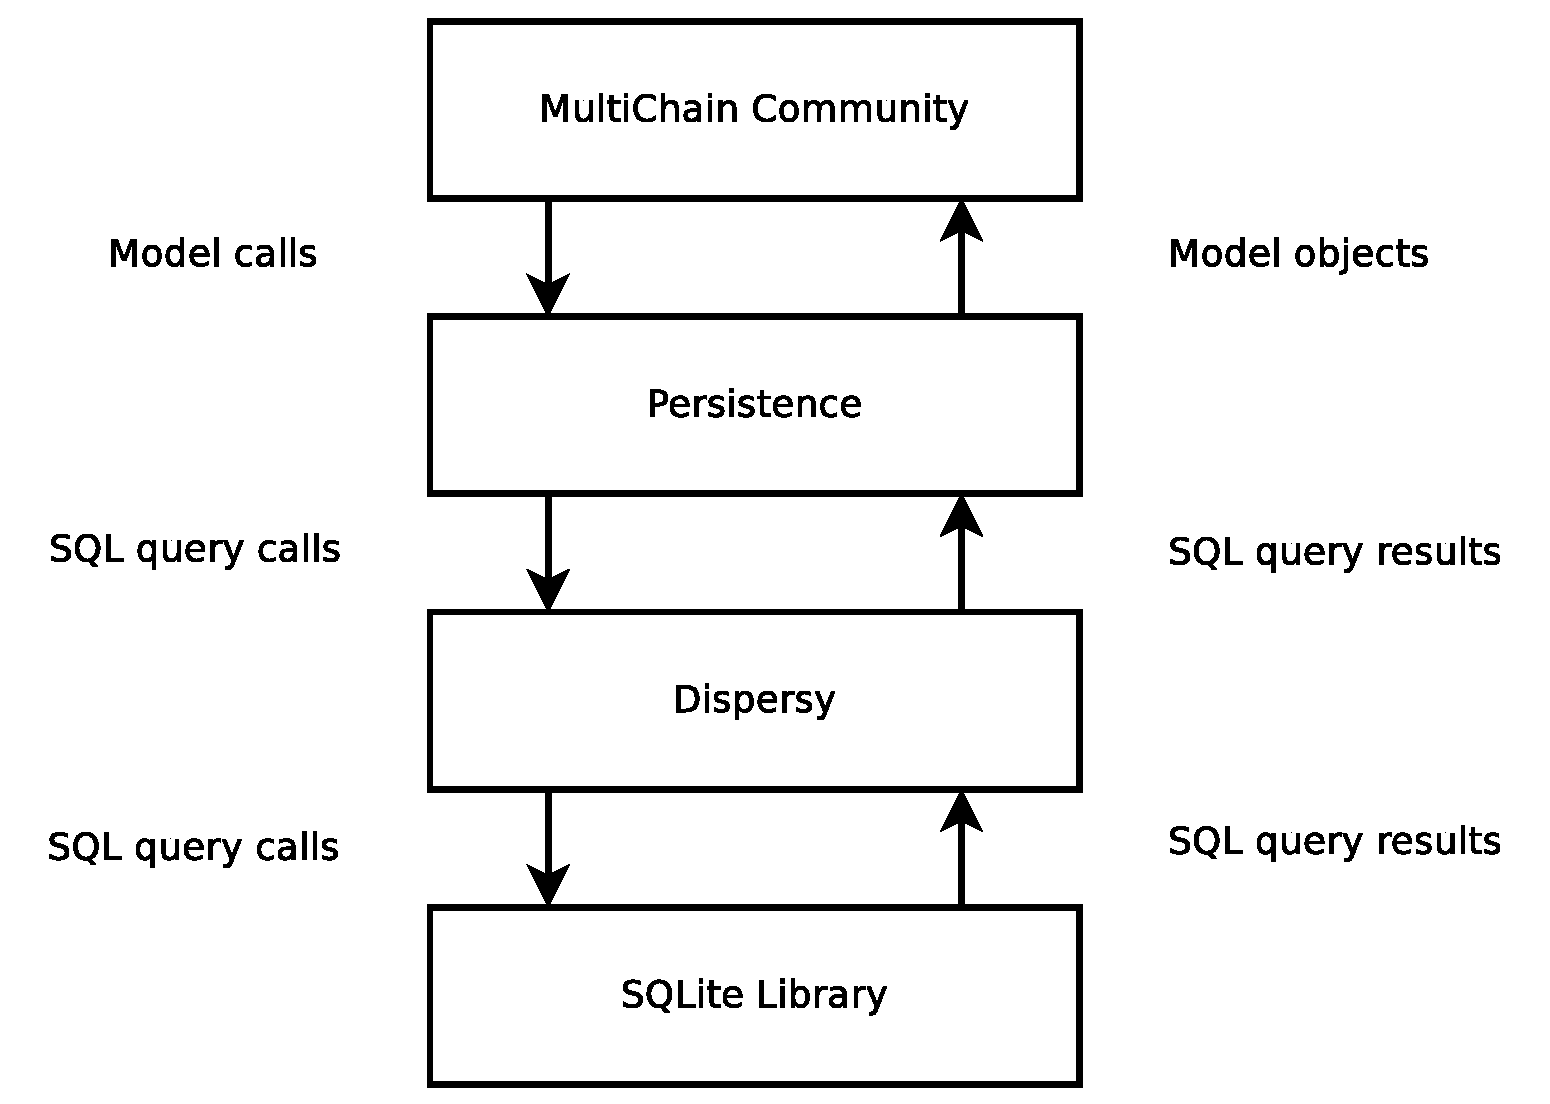
\includegraphics[scale=0.3]{design/figs/persistence-layer.eps}}
	\caption{Persistence layering in the software architecture}
	\label{fig:persistence-layer}
\end{figure}

The MultiChain Community calls functions in the persistence layer that have implicit knowledge about the model.
The Persistence layer formats SQL queries and passes these to the Dispersy layer.
The Dispersy layer performs several sanitation checks and passes these queries to the SQLite Library.
The SQLite Library and Dispersy layer both return the result of the SQL query.
These results are transformed by the Persistence layer into objects of the model usable by the MultiChain Community.

The only information that is saved are blocks.
The information all fits within one table.
A single block is saved as a single record called a row in a relation database.
Every attribute of a block is a single column in the row.
All attributes are saved directly into the database,
except for the public keys.
These public keys are hashed and these hashes are used as an identifier, called mid, in Dispersy.
The public keys are already saved in the Dispersy database.
When a block is retrieved from the database the public key is retrieved from Dispersy using the mid.

Every attribute is queryable in the database.
A public key can be converted to mid and is searched this way.
Every attribute is queryable to make the system  extensible
and usable when the next incremental steps are implemented.
It is presently unknown what information precisly will be needed,
so every information is now made available for the future.

\subsection{Dispersy database}
Dispersy keeps track of information on its own.
A record is kept of any message that can be retrieved using a message id.
The message is saved in a converted format and will be decoded when the message is retrieved.

Instead of storing information in a separate database,
the information could have been retrieved from the Dispersy database.
But the Dispersy database is not queryable.
Because all the information is stored in a converted format
that prevents queries to search the message for its contents.
For this reason, the dispersy database is not used and a separate database is used.

A future, possible improvement to Dispersy would be to save messages queryable in its database.
This would eliminate the current need for separate databases that contain aggregrated information.
The information is stored in two places within Tribler and this could be eliminated.
It would reduce the disk footprint and the amount of read/write transactions
as only one database would have to be maintained.
The I/O ineractions are a problem according to Tribler maintainers.

\section{Block size}
The size of a block is important as it determines how fast the total size of a chain will grow
and the utilization of the bandwidth of network to transfer blocks.
The size is dependend on the size of the parts of the blocks
and can be determined by the choice of cryptographic primitives.
Hashing function turn a variable message string to a fixed size message digest\cite{VanderLubbe-crypto}.
The fixed size is dependend on the choice of hashing function.
Similair cryptographic signing functions deterimine the size of a signature.
An overview of the size of the parts of a block can be seen in Table: \ref{table:block_size}.
The total size of a block is 296 bytes.

\begin{table}[]
\begin{adjustwidth}{-.5in}{-.5in}
\begin{center}
\begin{tabular}{lll||lll}
Name              & Type             & Bytes                   & Name              & Type             & Bytes \\ \hline
Uploaded MBytes   & unsigned integer & 4                       & Downloaded MBytes & unsigned integer & 4     \\
Total Up A        & unsigned integer & 8                       & Total Up B        & unsigned integer & 8     \\
Total Down A      & unsigned integer & 8                       & Total Down B      & unsigned integer & 8     \\
Prior Record A    & SHA1 digest      & 20                      & Prior Record B    & SHA1 digest      & 20    \\
Sequence Number A & signed integer   & 4                       & Sequence Number B & signed integer   & 4     \\
Public Key A      & EC key           & 64                      & Public Key B      & EC key           & 64    \\
Signature A       & EC signature     & 40                      & Signature B       & EC signature     & 40    \\ \hline
Total             &                  & 148                     & Total                  &                  & 148

\end{tabular}
\caption{Block subcomponents size.}
\label{table:block_size}
\end{center}
\end{adjustwidth}
\end{table}

An overview of every attribute and the size of the attribute inside the database can be seen in Table \ref{table:block_size_persistence}.
SQLite can grow the size of integers in its database to fit the required size
and therefore it can be in the range of $1,2,3,4$ bytes.
Because of this dynamic allocation and because public keys are stored in the Dispersy database
the total size is smaller.

\begin{table}[]
\begin{adjustwidth}{-.5in}{-.5in}
\begin{center}
\begin{tabular}{lll||lll}
Name              & Type             & Bytes                  & Name              & Type             & Bytes    \\ \hline
Uploaded MBytes   & unsigned integer & 1,2,4                  & Downloaded MBytes & unsigned integer & 1,2,4    \\
Total Up A        & unsigned integer & 1,2,4,8                & Total Up B        & unsigned integer & 1,2,4,8  \\
Total Down A      & unsigned integer & 1,2,4,8                & Total Down B      & unsigned integer & 1,2,4,8  \\
Prior Record A    & SHA1 digest      & 20                     & Prior Record B    & SHA1 digest      & 20       \\
Sequence Number A & signed integer   & 4                      & Sequence Number B & signed integer   & 4        \\
Mid A             & SHA1 digest      & 20                     & Mid B             & SHA1 digest      & 20       \\
Signature A       & EC signature     & 40                     & Signature B       & EC signature     & 40       \\ \hline
Total (min,max)   &                  & 87,104                 & Total (min,max    &                  & 87, 104
\end{tabular}
\caption{Block subcomponents size inside the database.}
\label{table:block_size_persistence}
\end{center}
\end{adjustwidth}
\end{table}

\subsubsection{Upper limit uploaded and downloaded MB}
The maximum integer size of the total up and total down impose an upper limit
on the total uploaded and downloaded MB that MultiChain can track.
This limit is imposed by SQLite and is $2^{62}$.
Bigger numbers cannot be saved in SQLite using a native datatype.
The upper limit for MultiChain is therefore 4.612 \ensuremath{\times 10^{9}} petabytes.
This is clearly more than sufficient for now.

\section{Integration with Tribler}
For integration a scheduler is implemented between the MultiChain community
and other parts of Tribler.
The scheduler tracks session upload and download amounts and schedules a block to be created,
when the amount of uploaded bytes is above a certain threshold.
The scheduler currently only tracks traffic of anonymous downloads.
Bartercast is not yet removed and
currently MultiChain runs together with Bartercast until MultiChain fully replaces Bartercast.

We recommend that the scheduler should be expanded to schedule blocks in a more sophisticated way.
The functionality of the scheduler is very limited and is missing basic functionality.
The most important improvement that should be introduced is the punishment of not signing blocks.
Currently, nodes can deny to have their behaviour tracked.
The next improvement is to actually determine the level of cooperation a node receives based upon their previous behaviour.
The actual decision making based upon past behaviour is not part of the thesis.
The processes of actually making the descision is a complicated process that has to take into account a lot of variables
and requires extensive experimentation to validate.
\section{Crawler}
We implemented a crawler that visits other nodes and request the full chain of that node.
The crawler was built to be used for the experiments and
is a first step in a more sophisticated crawler that will help to solve the known vulnerabilities.
These vulnerabilities will be described in chapter \ref{problems}.

\subsection{Recursively request blocks}
Dispersy provides a list of other nodes that were recently found
and can report when the node itself is found by another node.
Both are sources of destinations nodes that the crawler will visit
and request the chain from.

The crawler will first request from a node the block with sequence number $-1$.
This denotes that he wants the latest block in his chain.
The node returns this block to the crawler.
The crawler will persist the block if it is not yet know.

The newly retrieved block is chained to two blocks with the previous hashes.
The crawler will check if these blocks are present in the database.
If any block is not present,
then the crawler will request that particulair block.
The peer, to whom the block belongs to, has to be known in Dispersy.
If the peer is not known, the block is ignored.
This is done recursively untill the crawler reaches the genesis block of the chain.
In this fashion a breadth first search is implemented for any unknown block
that is present in the chain before the latest block.

The crawl tries to aggregrate as much blocks as possible.
But it gives no certainty that the full MultiChain is collected.
The crawler is able to crawl a disconnected MultiChain,
if for every disconnected partition a peer is known by Dispersy.

\begin{figure}
	\centerline{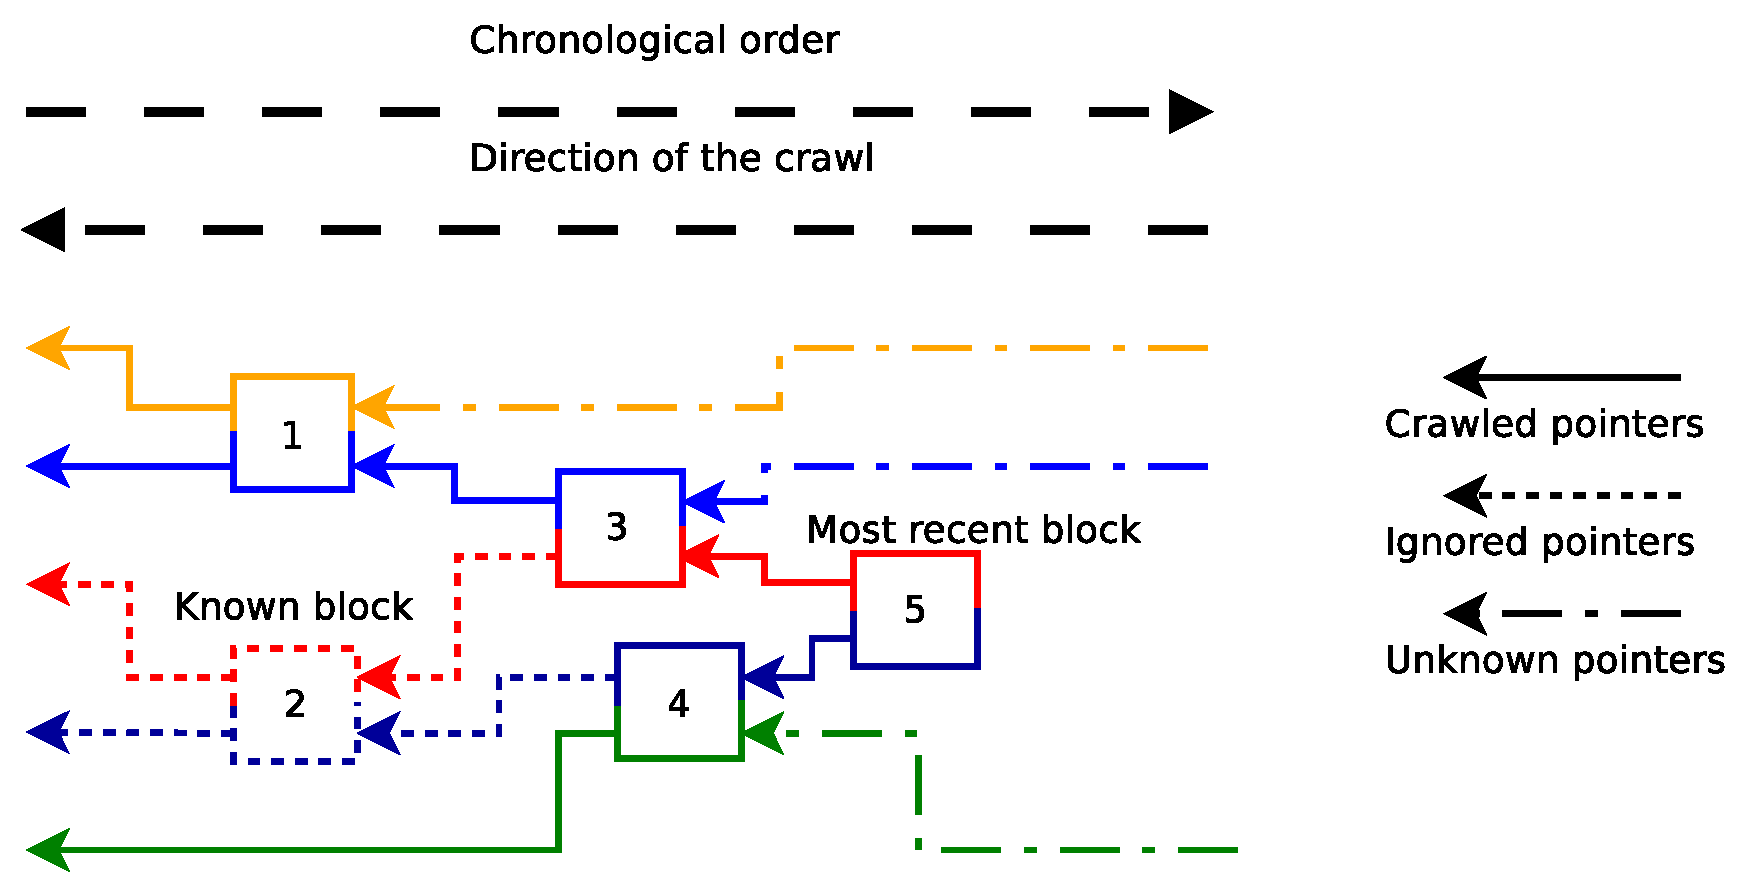
\includegraphics[scale=0.3]{design/figs/crawler-version2.eps}}
	\caption{Example of the crawler looking for unknown blocks. The crawler retrieves the most recent block and crawls older blocks.}
	\label{fig:crawler-example}
\end{figure}

An example can be seen in Figure \ref{fig:crawler-example}.
In this example the line arrows denote paths that the crawler follows,
dotted lines are paths that the crawler ignores,
half dotted lines are paths that the crawler will not know about.
Block 2 is already known by the crawler.
Block 5 is retrieved first by the crawler and the crawler sees hash links to block 3 and 4.
These are retrieved and the block finds links to block 1 and 2.
Because block 2 is already known, it is ignored.
Only block 1 is retrieved.
The crawler continues to follow the links further outside the displayed example.
The half dotted lines are not know by the crawler untill a block is retrieved that contains these paths.
The crawler will retrieve these blocks if for example the most recent block is requested.

\subsection{Recreation over retransmission}
An effort was made to try to reuse code of the community for the crawler and to not introduce another payload type in the community.
The attempt would reuse payload classes and authentication classes already used in the community for the creation of blocks.
This effort failed, because Dispersy cannot handle recreation of messages well
and would invalidate blocks that were recreated.

As said before, Dispersy also keeps tracks of messages received.
The messages containing a block requested by the crawler could be retrieved and retransmissioned forward
instead of being retrieved from the MultiChain database itself.
This would eliminate the need to construct a message and encode the message before it could be send,
because the encoded format is saved and can be retrieved and send immediately.
This was not used as it would be impossible to distinguish messages received as an response to a signature request or a crawler request.
The two types of responses cannot be processed in the same way.
A response to a signature requests has to influence the way a node responds to interactions
and a crawler response should not.

In the end, the crawler uses recreation of a block from the local database and uses a new payload type to forward blocks.
The main reasons this implementation was chosen is
that implemenation was very simple and had none of the above mentioned problems.
Maintainabillity is also much easier this way
as different types of messages are not using the same functions to be received in the code.
This might not be known by a new programmer working with the code.

\subsection{Improvements}
The crawler is a first, simple step towards a more sophisticated crawler.
Tribler has implemented already more sophisticated crawlers for Bartercast
and these techniques can be reused for the MultiChain crawler.
For example bloom filters can be used in conjunction with the knowledge
that every record is a part of the chain to quickly request multiple blocks\cite{broder-bloomfilter}\cite{logiotatidis-splash}.
Blocks could also be send in a more efficient way by sending multiple blocks per message.
Secondly, blocks that belong to a different node than the crawled node are requested,
but the location of this different node is only known by chance.
Dispersy only keeps track of 20 peers at any time, so the chance is low that the node is among these nodes.
The chance can be improved by asking if the first contacted node knows the location of the different node.



\section{Privacy}
Tribler has made an effort in providing a way for users to download anonymously and privately
~\cite{Plak-anonymous,ruigrok-anonymous,tanaskoski-anonymous}.
There is privacy in the contents of what is downloaded and anonimity in what is downloaded.
MultiChain should not leak information to break privacy and anonymity.

MultiChain only interacts with peers that are directly downloaded from or uploaded to.
With these peers blocks are created and transferred.
So anonymity is not broken by MultiChain.
An attacker could already analyse network traffic between these peers
and conclude they are downloading and uploading to each other.
But Tribler does not guarantee anonymity for this.
So MultiChain does not break anonymity with its interactions with peers.

A block only transcribe the amount of data that has been transferred between peers.
The content of the actual data is not transcribed.
The block also does not leak information of how big a single, individual transfer is between peers.
The amounts are aggregrated over all transfers.
The blocks also does not break the privacy.
Network analysis can already measure the total amount of data transferred.
So the design and implementation of MultiChain does not break anonymity already guaranteed by Tribler.

But MultiChain does make network analysis easier as measurement points between every node do not have to be introduced.
The chain of every node can be requested.
The chain contains the data of every transaction of a peer and can be used to analyse the network.
The network analysis can now also be performed retrospectively using data acquired from the MultiChain.

A reputation system can improve privacy.
The reputation system can be used to indentify nodes with high flow of data traffic.
These nodes can be used as a hop to send data to a destination.
Because the nodes have more cover traffic, they will provide more privacy\cite{acquisti-economics}.
In the absense of high traffic and high collaboration MultiChain should balance punishment of freeriding
with the wish for using the freeriding traffic as cover traffic to increase privacy\cite{dingledine-reputation}.

In the future we recommend to be able to transfer reputation using cryptographic functions in a new type of block: a transfer block.
This transfer block identifies a portion of reputation to transfer from one entity to another.
This make the reputation fungible and provide better safegaurds~\cite{acquisti-economics}, like forward anonymity.
Reputation can be earned and spend in an other place.
Reputation mining can be performed by collaborating with other peers.



